

\documentclass[12pt]{article}
\usepackage{graphicx}
\usepackage{amsmath}
\usepackage{listings}
\usepackage{color}
\usepackage[section]{placeins} %this stops the figures from showing up in wrong section

\definecolor{dkgreen}{rgb}{0,0.6,0}
\definecolor{dkblue}{rgb}{0,0.0,0.6}
\definecolor{dkred}{rgb}{0.9,0.0,0.1}


\begin{document}

\lstset{language=Fortran,tabsize=4,numbers=left,numberstyle=\tiny,basicstyle=\ttfamily\small\color{dkblue},stringstyle=\ttfamily\color{blue},keywordstyle=\rmfamily\color{dkred}\bfseries\emph,backgroundcolor=\color{white},commentstyle=\color{dkgreen}}




\title{Physics 562 - Computational Physics\\[.5cm]
Assignment 2: Quantum Harmonic Oscillator}
\author{Josh Fernandes\\
Department of Physics \& Astronomy\\
California State University Long Beach}
\date{\today}

  
\maketitle



\begin{abstract}
The assignment focuses on solving for the eigenfunctions for the one dimensional quantum harmonic oscillator. In the process, programs to imitate the exponential function, hermit function, and factorial function are created. The ground state and the first six excited states are plotted on a graph. The results are not normalized, so this paper only concludes that the amplitude decreases and the wavelength decreases as the energy state is increased.
\end{abstract}

\section{Introduction}\label{s:intro}

While the classical harmonic oscillator is well suited for solving systems of mechanical springs and pendulums, the quantum harmonic oscillator can solves systems of atomic particles. In addition, the quantum harmonic oscillator is one of the few quantum mechanical systems that has an exact, analytical solution. The eigenfunctions for the quantum harmonic oscillator are of the form

\begin{gather}
\Psi_n(x) = \frac{1}{\sqrt{2^n \, n!}}\cdot \left(\frac{mw}{\pi \hbar}\right)^{\frac{1}{4}} \cdot e^{-\frac{mwx^2}{2\hbar}} \cdot H_n \left(\sqrt{\frac{mw}{\hbar}} \, x \right).
\end{gather}

The parameters are set as $m=1$, $w=1$, and $\hbar=3$. Although these values have no physical meaning, they preserve the shape of the curves. The first seven energy states are plotted in order to determine traits about the curves.
\section{The Fortran95 code}

The Makefile in Listing \ \ref{makefile} describes the structure of the code. The codes in {\tt OBJS1} are 
compiled together. The {\tt .o} files were created from the {\tt .f95} file by using the {\tt F95} command
with flags {\tt F95FLAGS}. In building the executable code {\tt LDFLAGS} were used, which contains 
the {\tt LIB} library. These {\tt LDFLAGS} are optimal for Intel Core2 architecture and uses the 
Apple's {\tt vecLib} library from Xcode. By typing {\tt make} we can produce the executable file.





\begin{lstlisting}[frame=single,caption={The {\tt Makefile}},label=makefile]

OBJS = numtype.o oscillator.0 

PROG = wowza

F95 = gfortran

F95FLAGS = -O3 -funroll-loops -fexternal-blas

LIBS = -framework vecLib

LDFLAGS = $(LIBS)

all: $(PROG) 

$(PROG): $(OBJS)
	$(F95) $(LDFLAGS) -o $@ $(OBJS) 

clean:
	rm -f $(PROG) *.{o,mod}

.SUFFIXES: $(SUFFIXES) .f95

.f95.o:
	$(F95) $(F95FLAGS) -c $<

\end{lstlisting}

The Fortran95 code is shown below. The precision is defined in the Module {\tt NumType}. The constants parameters are defined in Module {\tt setup}. The implicit none statement ensures that all the variables has to be defined. {\tt do while} is used to increase the value of x while also calculating $\Psi$ for the eight different $n$ values. The resulting wave functions are plotted with an offset on the y axis so they can be clearly seen. A horizontal line is plotted at the offset for clarity using the arrays $plot1$ through $plot8$. The function {\tt contains} is a way of defining a function that can be reused within the code. In this code, three different functions are defined. Note that in each function, the variables that are used have to be defined.   


\begin{lstlisting}[frame=single,caption={Module {\tt NumType}},label=module]

module NumType

	save
	integer, parameter :: dp = kind(1.d0)
	real(dp), parameter :: pi = 4*atan(1._dp), &
	e = exp(1._dp)
	complex(dp), parameter :: iic = (0._dp,1._dp)
	
end module NumType

\end{lstlisting}


\begin{lstlisting}[frame=single,caption={{\tt oscillator.f95}},label=scattering95]

module initiate_phase_one

	use NumType
	implicit none
	real(dp), parameter :: w = 1._dp, &
	m = 1._dp, Xmin = -10._dp, Xmax = 10._dp
	real(dp) :: x, k, plot1(5000),plot2(5000),&
	plot3(5000), plot4(5000),plot5(5000), &
	plot6(5000),plot7(5000), plot8(5000)
	REAL, DIMENSION(:, :), ALLOCATABLE :: psi
	integer, Dimension(:), ALLOCATABLE :: n
	real(dp), Dimension(:), ALLOCATABLE :: curve
	integer :: i, j, DeAllocateStatus, & 
	AllocateStatus, steps
	

end module initiate_phase_one

program awesome

	use initiate_phase_one
	
	n = (/0,1, 2, 3, 4, 5, 6, 7/)

	j = 0._dp
	k = 0.5_dp

	steps = 5000
	x = Xmin
	dx = (Xmax-Xmin)/steps



	ALLOCATE (curve(steps), STAT = AllocateStatus)
	IF (AllocateStatus /= 0) & 
	STOP "*** Not enough memory ***"

	ALLOCATE ( psi(size(n), steps), STAT = AllocateStatus)
	IF (AllocateStatus /= 0) &
	STOP "*** Not enough memory ***"

	do while(x < Xmax)
		j = j + 1
		curve(j) = 0.5_dp*k*x**2
		plot1(j) = 1
		plot2(j) = 3
		plot3(j) = 5
		plot4(j) = 7
		plot5(j) = 9
		plot6(j) = 11
		plot7(j) = 13
		plot8(j) = 15
		do i=1,size(n)
			psi(i,j) = quantum_oscillator(n(i),m,w,x)
		end do
		print *, x, 1+psi(1,j), 3+psi(2,j), &
		5+psi(3,j), 7+psi(4,j), 9+psi(5,j), &
		11+psi(6,j), 13+psi(7,j), 15+psi(8,j), &
		curve(j), plot1(j), plot2(j), plot3(j), &
		plot4(j), plot5(j), plot6(j), plot7(j), plot8(j)
		!iterate x
		x = x + dx
	end do

	DEALLOCATE (curve, STAT = DeAllocateStatus)
	DEALLOCATE (psi, STAT = DeAllocateStatus)


	

	contains

		function quantum_oscillator(n,m,w,x) result(psi)

			implicit none
			real(dp), parameter :: hbar = 3._dp
			real(dp) :: m,w,x,psi
			integer :: n

			psi = 1/sqrt(real((2**n)*factorial(n)))*&
			((m*w)/(pi*hbar))**(1/4)&
			*exxp(-(m*w*x**2)/(2*hbar))*&
			hermite(n,(sqrt(m*w/hbar)*x))

		end function quantum_oscillator

		recursive function exxp(x) result(ex)

		real(dp) :: x, ex, E0
		integer :: i, imax

		imax = 20
		if ( abs(x) < 1._dp) then
			E0 = 1._dp
			ex = 1._dp
			do i =1, imax
				E0 = E0*x/i
				ex = ex + E0
			end do
		else if (1._dp <= x) then
			ex = e * exxp(x-1)
		else if (x <= 1._dp) then
			ex = exxp(x+1) / e
		end if

		end function exxp 

		recursive function hermite(n,x) result(hpol)

			real(dp) :: x, hpol
			integer :: n

			if ( n < 0 ) then
				stop "n can't be less than zero"
			else if ( n == 0) then
				hpol = 1._dp
			else if ( n == 1) then
				hpol = 2*x
			else
				hpol = 2*x*hermite(n-1,x) - &
				2*(n-1)*hermite(n-2,x)
			end if 


		end function hermite


		recursive function factorial(n) &
		result(factorial_number)

			implicit none
			integer :: n, factorial_number


			if ( n < 0 ) then
				stop "you know that's wrong"
			else if ( n == 0) then
				factorial_number = 1
			else
				factorial_number = n*factorial(n-1)
			end if 



		end function factorial


end program awesome

\end{lstlisting}


The code is run by typing {\tt ./wowza}. The results are printed on the screen, or the data can redirect to the file {\tt amazing data} by typing {\tt ./wowza > amazingdata.data}. The {\tt Plot} provides the picture in Fig.\ \ref{linearscattering}. 


\begin{figure}[!htb]
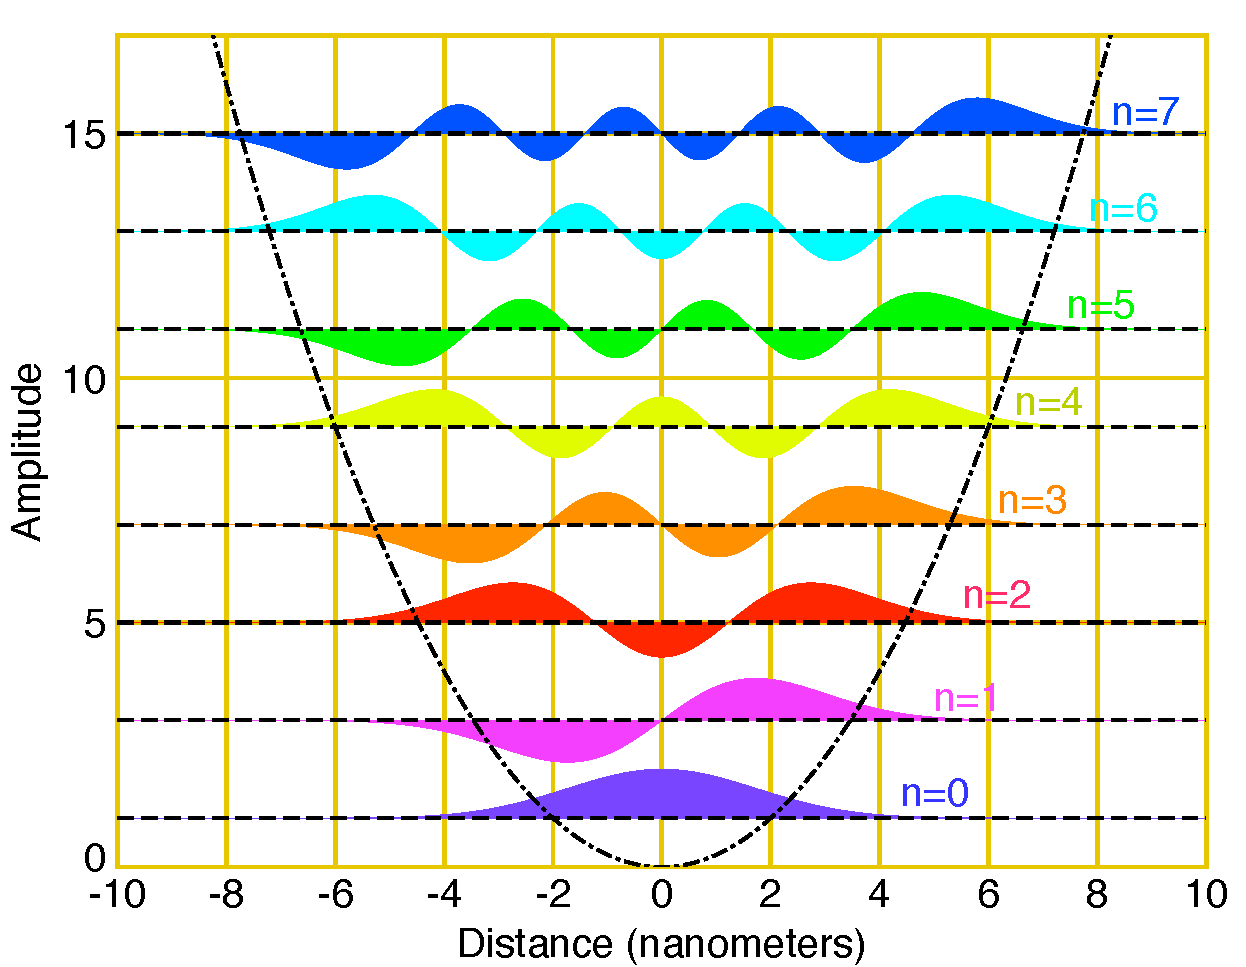
\includegraphics[width=1.\textwidth]{quantum_oscillator.pdf}
\caption{Results of the {\tt oscillator.f95} code plotted on a linear scale. }
\label{linearscattering}
\end{figure}





\section{Summary and conclusions}

The eigenfunctions $\Psi$ for the first eight energy states were plotted. The graph demonstrates that as $n$ increases the amplitude decreases and the wavelength decreases.

\begin{thebibliography}{}


\bibitem{metcalf} M.\ Metcalf, J.\ Reid and M.\ Cohen, {\it Fortran 95/2003 explained}. Oxford University Press, 2004.
 

\end{thebibliography}




\end{document}
